\documentclass{article}
\usepackage[spanish]{babel}
\usepackage{fancyhdr}
\usepackage{graphicx}
\usepackage{setspace}
\usepackage[table]{xcolor}
\usepackage{tabularx}
\usepackage{array}
\usepackage{multicol}
\usepackage{multirow}
\usepackage[margin=2.5cm]{geometry}
\usepackage{float}
\usepackage{color, colortbl}
\definecolor{tablebackground}{rgb}{0.8, 0, 0}


\newcolumntype{M}[1]{>{\centering\arraybackslash}m{#1}}
\newcolumntype{N}{>{\centering\arraybackslash}p{3.5cm}}
\newcolumntype{x}[1]{>{\centering\arraybackslash}p{#1}}

\pagestyle{fancy}
\lhead{\begin{picture}(0,0) \put(0,0){
\includegraphics[width=30mm]{img/logoSistemas.png}} \end{picture}}
\rhead{\begin{picture}(0,0) \put(-33,5){
\includegraphics[width=12mm]{./img/logoAbet.png}} \end{picture}}
\renewcommand{\headrulewidth}{0.5pt}

\fancyhead[C]{
 	\tiny Universidad Nacional de San Agustín de Arequipa \\
  	Facultad de Ingeniería de Producción y Servicios \\
  	Departamento de Ingeniería de Sistemas e Informática \\
  	Escuela Profesional de Ingeniería de Sistemas \\
  	\textbf{Programación Web 2}
}

\fancyfoot[L]{Estudiante Rafael Nina Calizaya}
\fancyfoot[C]{Pag. \thepage}
\fancyfoot[R]{Programación Web 2}
\renewcommand{\footrulewidth}{0.5pt}


\newcommand{\itemNombre}{Rafael Diego Nina Calizaya}
\newcommand{\itemCorreo}{rninacal@unsa.edu.pe}
\newcommand{\itemEscuela}{Escuela Profesional de Ingeniería de Sistemas}
\newcommand{\itemCurso}{Programación Web 2}
\newcommand{\itemSemestre}{III}
\newcommand{\itemCodigo}{1702122}
\newcommand{\itemLaboratorio}{03}
\newcommand{\itemTema}{JavaScript}
\newcommand{\itemSemestreAcademico}{2024-A}
\newcommand{\itemInicio}{13 Mayo 2024}
\newcommand{\itemFinal}{17 Mayo 2024}

\begin{document}
.

\begin{center}	
	\fontsize{17}{17} \textbf{ Informe de Laboratorio \itemLaboratorio}
\end{center}
\centerline{\textbf{\Large Tema: JavaScript}}

\begin{flushright}
	\begin{tabular}{|M{2.5cm}|N|}
		\hline
		\rowcolor{tablebackground}
		\color{white} \textbf{Nota}  \\
		\hline 
		     \\[18pt]
		\hline 			
	\end{tabular}
\end{flushright}	
\begin{table}[h]
	\renewcommand{\arraystretch}{0.5}
	\hspace{2px}
	\begin{tabular}{|x{4.8cm}|x{4.8cm}|x{4.8cm}|}
		\hline 
		\rowcolor{tablebackground}
		\color{white} \textbf{Estudiante} & \color{white}\textbf{Escuela}  & \color{white}\textbf{Asignatura}   \\
		\hline 
		{\itemNombre \par \itemCorreo} & \itemEscuela & {\itemCurso \par Semestre: \itemSemestre \par Código: \itemCodigo}     \\
		\hline 			
	\end{tabular}
\end{table}		
	
\begin{table}[h]
	\renewcommand{\arraystretch}{0.5}
	\hspace{2px}
	\begin{tabular}{|x{4.8cm}|x{4.8cm}|x{4.8cm}|}
		\hline 
		\rowcolor{tablebackground}
		\color{white}\textbf{Laboratorio} & \color{white}\textbf{Tema}  & \color{white}\textbf{Duración}   \\
		\hline 
		\itemLaboratorio & \itemTema & 06  \\
		\hline 
	\end{tabular}
\end{table}

\begin{table}[h]
	\renewcommand{\arraystretch}{0.5}
	\hspace{2px}
	\begin{tabular}{|x{4.8cm}|x{4.8cm}|x{4.8cm}|}
		\hline 
		\rowcolor{tablebackground}
		\color{white}\textbf{Semestre académico} & \color{white}\textbf{Fecha de inicio}  & \color{white}\textbf{Fecha de entrega}   \\
		\hline 
		\itemSemestreAcademico & \itemInicio &  \itemFinal  \\
		\hline 
	\end{tabular}
\end{table}

\section{URL del Repositorio:}
https://github.com/DrN25/pw2\_24a/tree/main/Lab03
	
\section{Tarea:}
Se busca programar en JavaScript sobre una página web html básica.
\subsection*{Ejercicio 01: Teclado random para Banca por Internet.}
Se crearon varias funciones para ello, entre ellas tenemos:
\begin{itemize}
    \item \textbf{teclado(): } Esta función se encarga de generar el teclado de la banca, la cual asignará 1 valor a cada uno de los 10 botones numéricos, y cuando sean presionados el valor del cuadro de la derecha se actualizará. En caso se seleccione el botón Limpiar se borrará lo escrito.\\



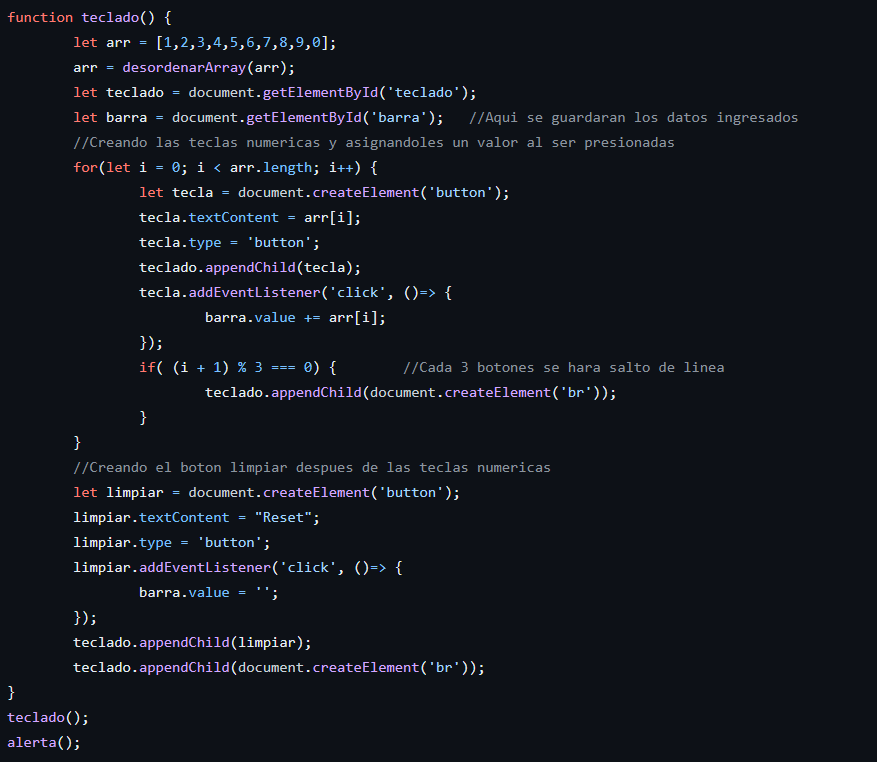
\includegraphics[width=\textwidth]{img/2.png}
\item \textbf{desordenarArray(): } Esta función se encarga de desordenar el arreglo enviado. Su objetivo es que cada vez que se actualice la página o se envíen los datos, se llame a esta función para que el orden de las teclas sea randomizado.\\



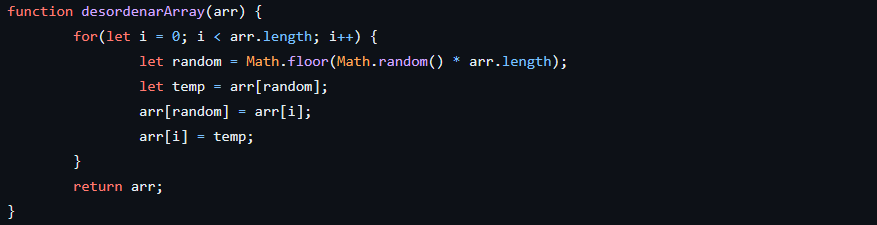
\includegraphics[width=\textwidth]{img/3.png}
\item \textbf{alerta(): } Esta función se encarga de mostrar un mensaje de alerta cuando se hayan enviado los datos correctamente.\\



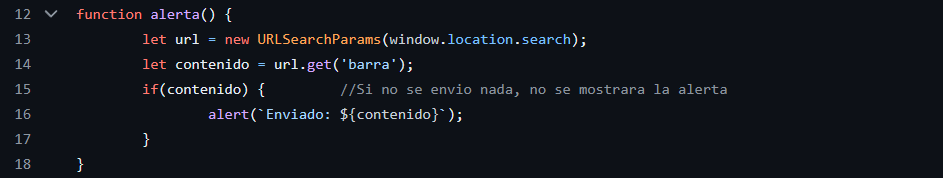
\includegraphics[width=\textwidth]{img/4.png}
\end{itemize}
Pagina Web Implementada.\\



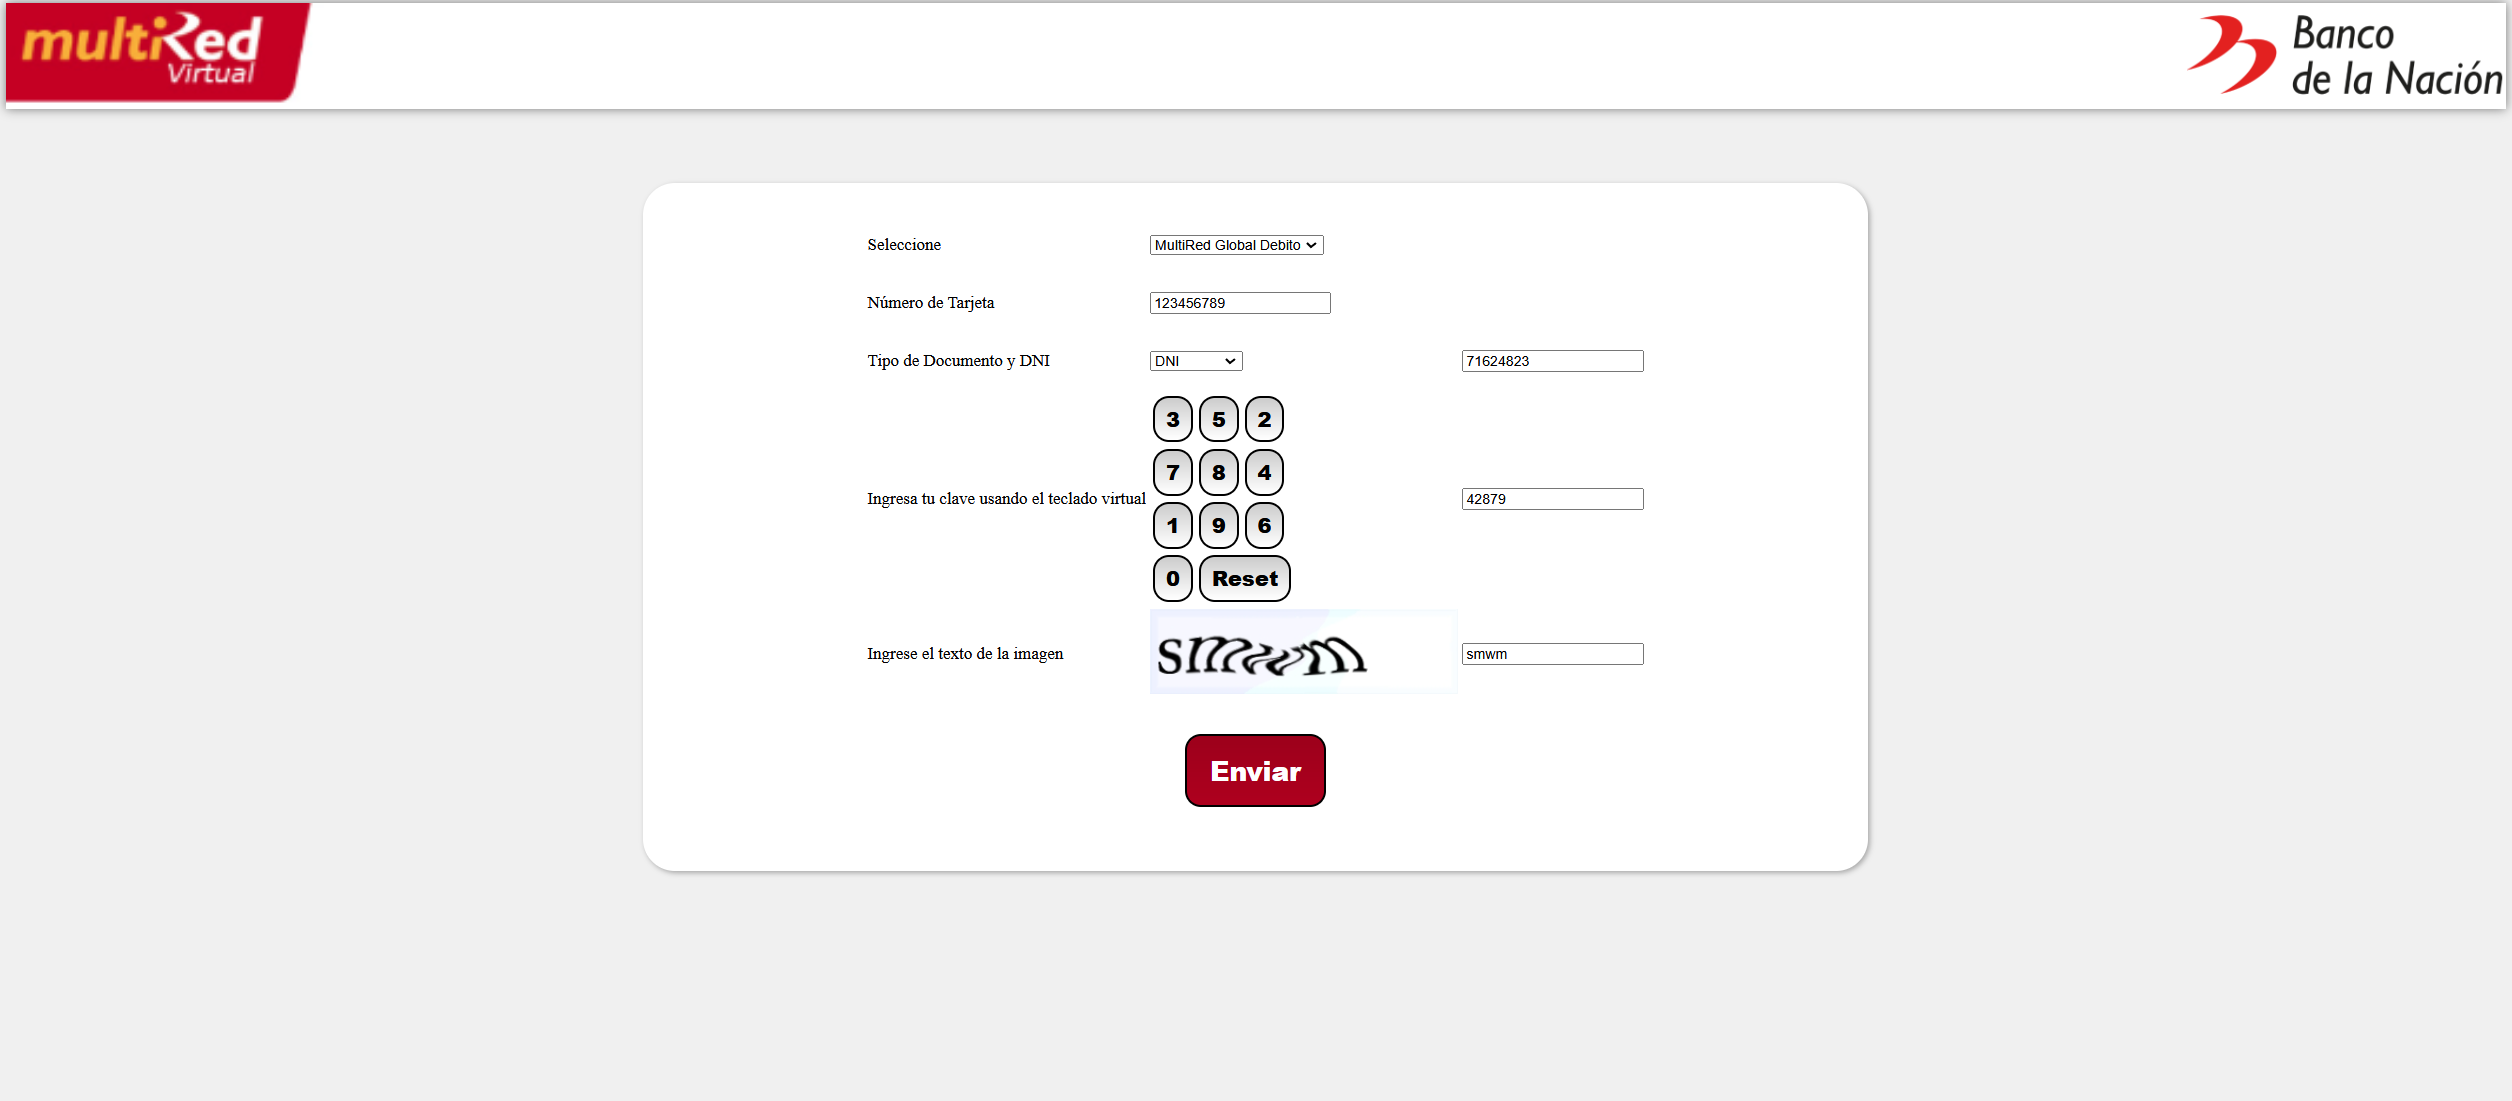
\includegraphics[width=\textwidth]{img/1.png}

\subsection*{Ejercicio 02: Calculadora.}
Para ello se creo una función:
\begin{itemize}
\item \textbf{calculadora(): } Esta función se encarga de generar los botones del teclado, incluyendo números y operaciones. Cada vez que se presione un número u operación se agregaran a la barra de resultados, pero cuando se presione en E se eliminara el último carácter, con C se elimina todo y con = se llama a la función eval(), dando error si no se puede dar la operación. En este también se almacenan las operaciones realizadas cada vez que se presiona el botón =.\\



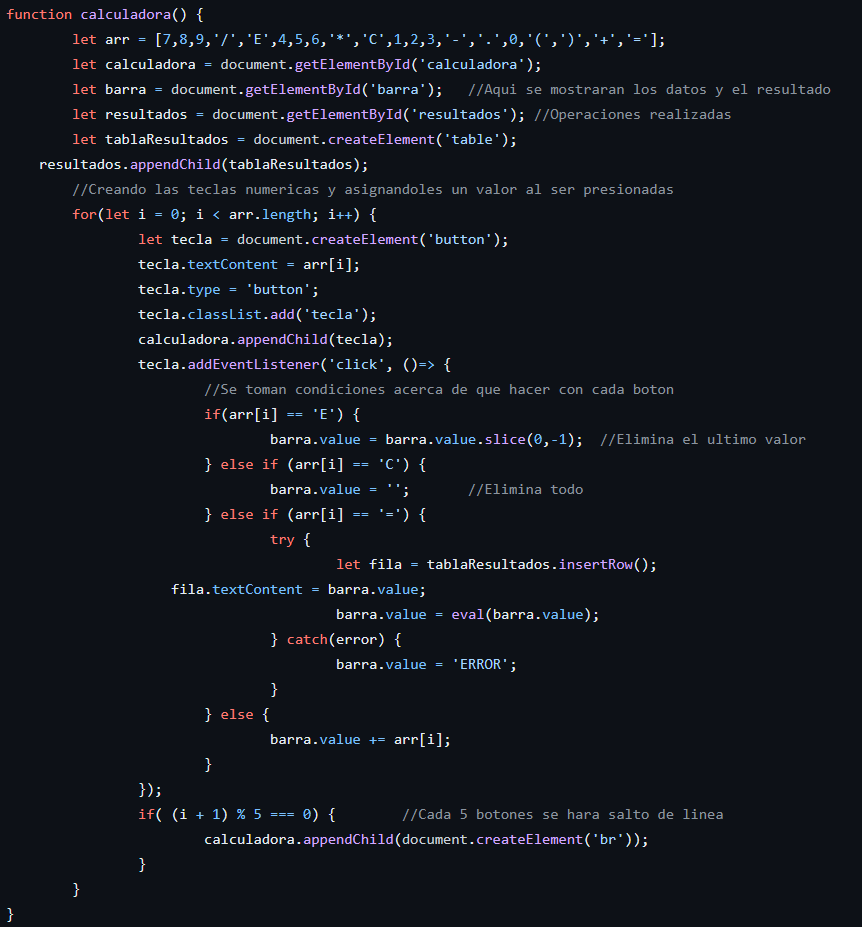
\includegraphics[width=\textwidth]{img/5.png}
\end{itemize}
Pagina Web Implementada.\\



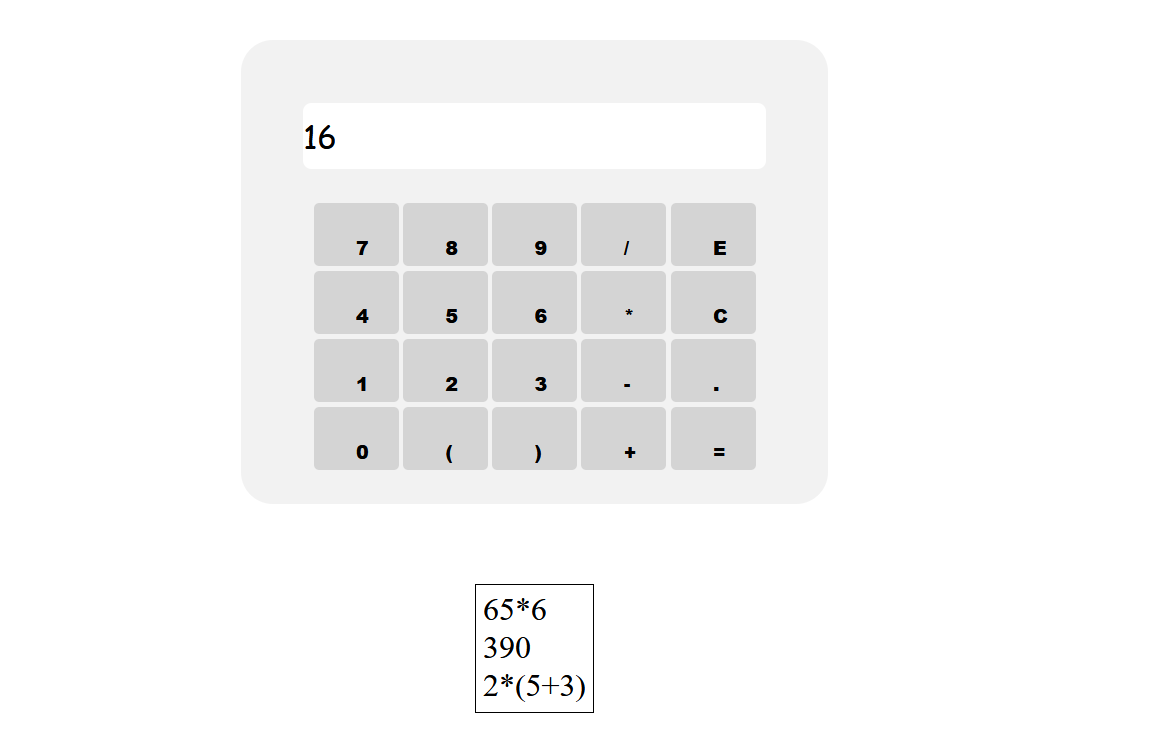
\includegraphics[width=\textwidth]{img/6.png}

\subsection*{Ejercicio 03: Juego el Ahorcado.}
Se crearon varias funciones para ello, entre ellas tenemos:
\begin{itemize}
\item \textbf{ahorcado(): } Esta función se encarga de generar los botones del abecedario para jugar, además de verificar la lógica del juego y aplicar un conteo de errores para cada intento del jugador, donde en caso de llegar a los 7 errores se mostrará un mensaje de que se perdió el juego.\\



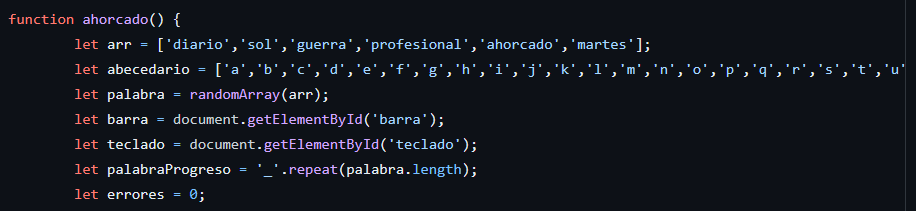
\includegraphics[width=\textwidth]{img/7.png}






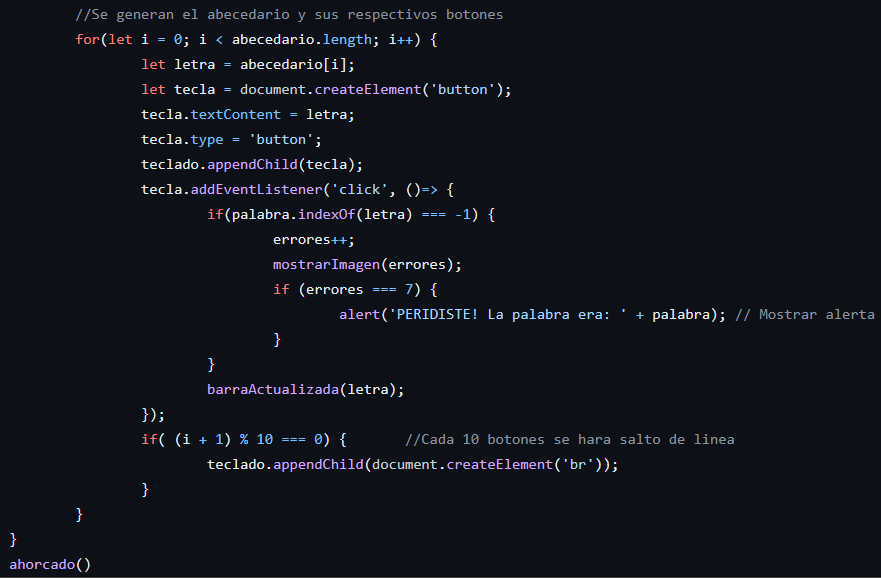
\includegraphics[width=\textwidth]{img/8.png}
\item \textbf{randomArray(): } Esta función se encarga de elegir de manera randomizada una de las palabras del arreglo entregado, la cual será usada durante todo el juego.\\



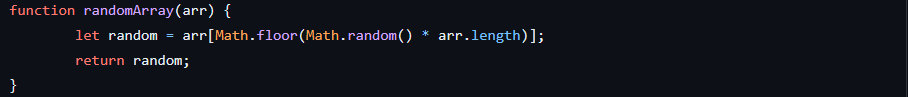
\includegraphics[width=\textwidth]{img/11.png}
\item \textbf{barraActualizada(): } Esta función se encarga de actualizar la barra en la cual se mostrará el avance del juego cada vez que se presione una tecla. Al inicio se imprimirán únicamente -, y cuando se adivine una letra se reemplaza esta letra en la barra.\\



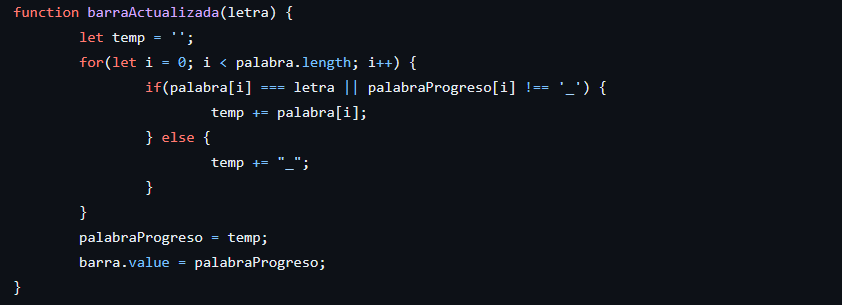
\includegraphics[width=\textwidth]{img/9.png}
\item \textbf{mostrarImagen(): } Esta función se encarga de actualizar la imagen del ahorcado cada vez que haya un error en cada intento.\\



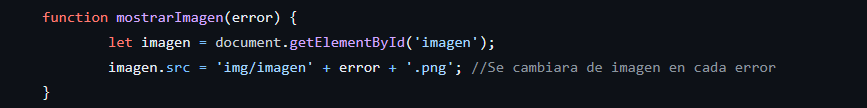
\includegraphics[width=\textwidth]{img/10.png}
\end{itemize}
Pagina Web Implementada.\\



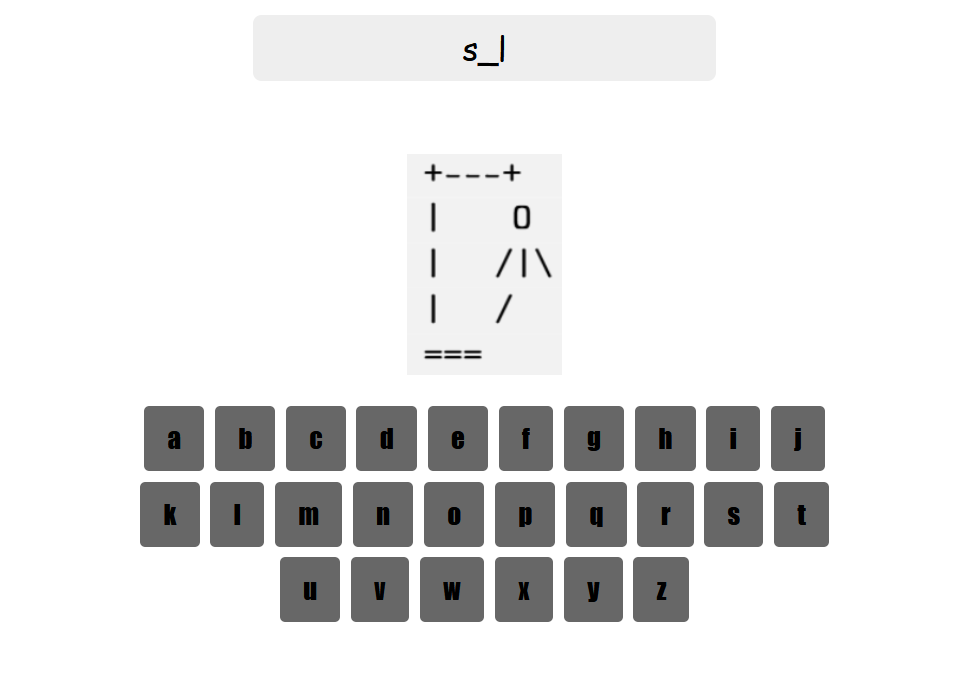
\includegraphics[width=\textwidth]{img/12.png}
\section{Commits Realizados:}




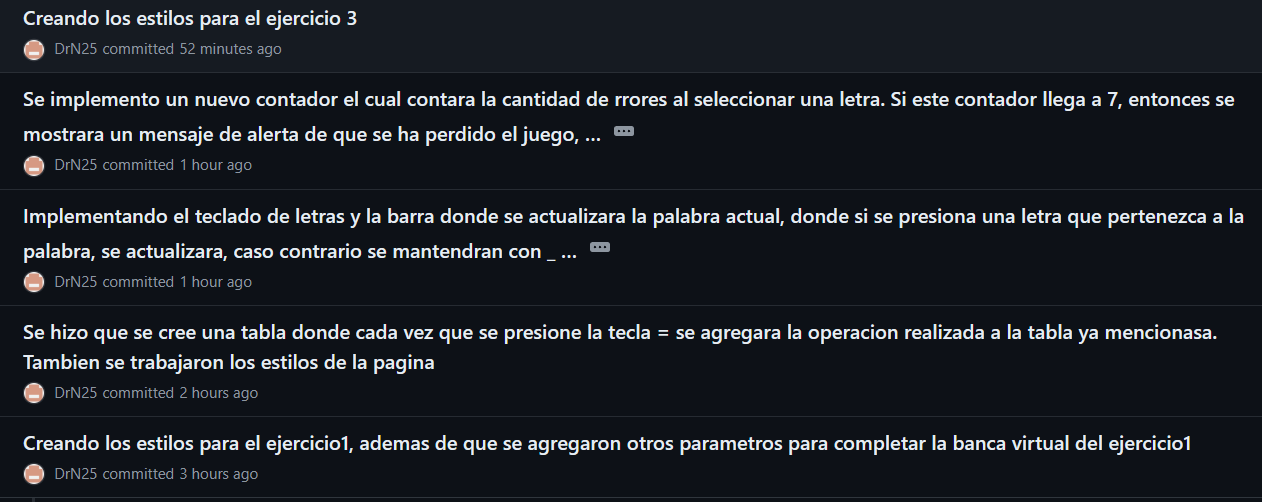
\includegraphics[width=\textwidth]{img/14.png}




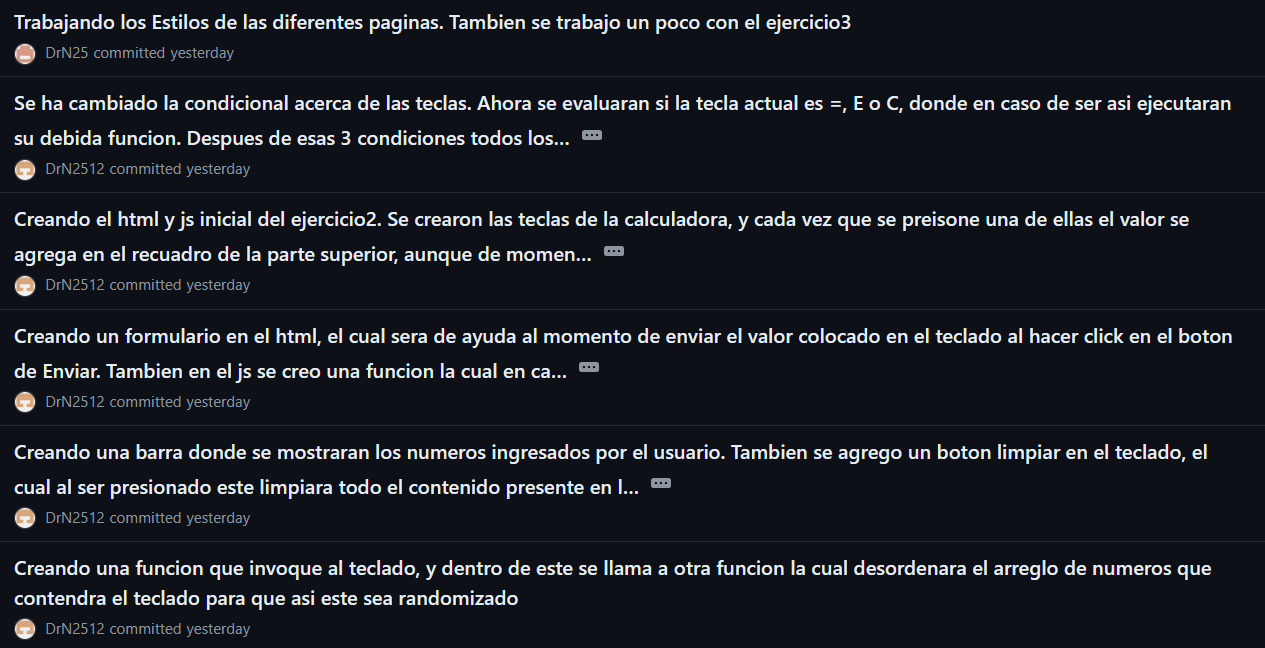
\includegraphics[width=\textwidth]{img/13.png}
\section{Rúbrica:}




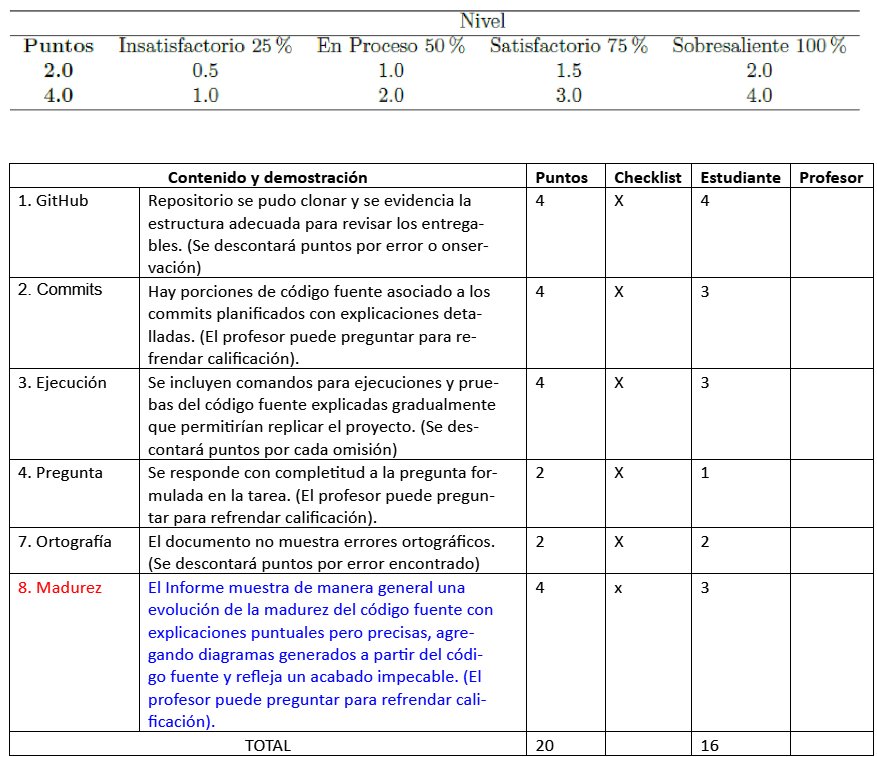
\includegraphics[width=\textwidth]{img/rubrica.png}
\end{document}